\documentclass[12pt]{article}
\usepackage[a4paper,margin=25mm]{geometry}
\usepackage{fontspec}
\setmainfont{TeX Gyre Pagella}
\usepackage{amsmath,amssymb,amsthm}
\usepackage{booktabs,array}
\usepackage{tikz}
\usetikzlibrary{arrows.meta,positioning}
\usepackage{hyperref}
\hypersetup{colorlinks=true,linkcolor=black,urlcolor=blue,citecolor=black}
\newtheorem{proposition}{Proposition}
\newcommand{\ket}[1]{\lvert #1\rangle}
\newcommand{\bra}[1]{\langle #1\rvert}
\newcommand{\tr}{\operatorname{tr}}
\newcommand{\ord}{\operatorname{ord}}
\newcommand{\id}{\operatorname{id}}
\newcommand{\W}{\mathsf{W}}
\newfontfamily\shavfont[Scale=1.0]{Trabajo}
\newfontface\igprimfont{Everson Mono}
\usepackage{newunicodechar}
\AtBeginDocument{
\newunicodechar{𐑐}{\ifmmode\text{{\shavfont 𐑐}}\else{{\shavfont 𐑐}}\fi}
\newunicodechar{𐑑}{\ifmmode\text{{\shavfont 𐑑}}\else{{\shavfont 𐑑}}\fi}
\newunicodechar{𐑒}{\ifmmode\text{{\shavfont 𐑒}}\else{{\shavfont 𐑒}}\fi}
\newunicodechar{𐑓}{\ifmmode\text{{\shavfont 𐑓}}\else{{\shavfont 𐑓}}\fi}
\newunicodechar{𐑔}{\ifmmode\text{{\shavfont 𐑔}}\else{{\shavfont 𐑔}}\fi}
\newunicodechar{𐑕}{\ifmmode\text{{\shavfont 𐑕}}\else{{\shavfont 𐑕}}\fi}
\newunicodechar{𐑖}{\ifmmode\text{{\shavfont 𐑖}}\else{{\shavfont 𐑖}}\fi}
\newunicodechar{𐑗}{\ifmmode\text{{\shavfont 𐑗}}\else{{\shavfont 𐑗}}\fi}
\newunicodechar{𐑘}{\ifmmode\text{{\shavfont 𐑘}}\else{{\shavfont 𐑘}}\fi}
\newunicodechar{𐑙}{\ifmmode\text{{\shavfont 𐑙}}\else{{\shavfont 𐑙}}\fi}
\newunicodechar{𐑚}{\ifmmode\text{{\shavfont 𐑚}}\else{{\shavfont 𐑚}}\fi}
\newunicodechar{𐑛}{\ifmmode\text{{\shavfont 𐑛}}\else{{\shavfont 𐑛}}\fi}
\newunicodechar{𐑜}{\ifmmode\text{{\shavfont 𐑜}}\else{{\shavfont 𐑜}}\fi}
\newunicodechar{𐑝}{\ifmmode\text{{\shavfont 𐑝}}\else{{\shavfont 𐑝}}\fi}
\newunicodechar{𐑞}{\ifmmode\text{{\shavfont 𐑞}}\else{{\shavfont 𐑞}}\fi}
\newunicodechar{𐑟}{\ifmmode\text{{\shavfont 𐑟}}\else{{\shavfont 𐑟}}\fi}
\newunicodechar{𐑠}{\ifmmode\text{{\shavfont 𐑠}}\else{{\shavfont 𐑠}}\fi}
\newunicodechar{𐑡}{\ifmmode\text{{\shavfont 𐑡}}\else{{\shavfont 𐑡}}\fi}
\newunicodechar{𐑢}{\ifmmode\text{{\shavfont 𐑢}}\else{{\shavfont 𐑢}}\fi}
\newunicodechar{𐑣}{\ifmmode\text{{\shavfont 𐑣}}\else{{\shavfont 𐑣}}\fi}
\newunicodechar{𐑤}{\ifmmode\text{{\shavfont 𐑤}}\else{{\shavfont 𐑤}}\fi}
\newunicodechar{𐑥}{\ifmmode\text{{\shavfont 𐑥}}\else{{\shavfont 𐑥}}\fi}
\newunicodechar{𐑦}{\ifmmode\text{{\shavfont 𐑦}}\else{{\shavfont 𐑦}}\fi}
\newunicodechar{𐑧}{\ifmmode\text{{\shavfont 𐑧}}\else{{\shavfont 𐑧}}\fi}
\newunicodechar{𐑨}{\ifmmode\text{{\shavfont 𐑨}}\else{{\shavfont 𐑨}}\fi}
\newunicodechar{𐑩}{\ifmmode\text{{\shavfont 𐑩}}\else{{\shavfont 𐑩}}\fi}
\newunicodechar{𐑪}{\ifmmode\text{{\shavfont 𐑪}}\else{{\shavfont 𐑪}}\fi}
\newunicodechar{𐑫}{\ifmmode\text{{\shavfont 𐑫}}\else{{\shavfont 𐑫}}\fi}
\newunicodechar{𐑬}{\ifmmode\text{{\shavfont 𐑬}}\else{{\shavfont 𐑬}}\fi}
\newunicodechar{𐑭}{\ifmmode\text{{\shavfont 𐑭}}\else{{\shavfont 𐑭}}\fi}
\newunicodechar{𐑮}{\ifmmode\text{{\shavfont 𐑮}}\else{{\shavfont 𐑮}}\fi}
\newunicodechar{𐑯}{\ifmmode\text{{\shavfont 𐑯}}\else{{\shavfont 𐑯}}\fi}
\newunicodechar{𐑰}{\ifmmode\text{{\shavfont 𐑰}}\else{{\shavfont 𐑰}}\fi}
\newunicodechar{𐑱}{\ifmmode\text{{\shavfont 𐑱}}\else{{\shavfont 𐑱}}\fi}
\newunicodechar{𐑲}{\ifmmode\text{{\shavfont 𐑲}}\else{{\shavfont 𐑲}}\fi}
\newunicodechar{𐑳}{\ifmmode\text{{\shavfont 𐑳}}\else{{\shavfont 𐑳}}\fi}
\newunicodechar{𐑴}{\ifmmode\text{{\shavfont 𐑴}}\else{{\shavfont 𐑴}}\fi}
\newunicodechar{𐑵}{\ifmmode\text{{\shavfont 𐑵}}\else{{\shavfont 𐑵}}\fi}
\newunicodechar{𐑶}{\ifmmode\text{{\shavfont 𐑶}}\else{{\shavfont 𐑶}}\fi}
\newunicodechar{𐑷}{\ifmmode\text{{\shavfont 𐑷}}\else{{\shavfont 𐑷}}\fi}
\newunicodechar{𐑸}{\ifmmode\text{{\shavfont 𐑸}}\else{{\shavfont 𐑸}}\fi}
\newunicodechar{𐑹}{\ifmmode\text{{\shavfont 𐑹}}\else{{\shavfont 𐑹}}\fi}
\newunicodechar{𐑺}{\ifmmode\text{{\shavfont 𐑺}}\else{{\shavfont 𐑺}}\fi}
\newunicodechar{𐑻}{\ifmmode\text{{\shavfont 𐑻}}\else{{\shavfont 𐑻}}\fi}
\newunicodechar{𐑼}{\ifmmode\text{{\shavfont 𐑼}}\else{{\shavfont 𐑼}}\fi}
\newunicodechar{𐑽}{\ifmmode\text{{\shavfont 𐑽}}\else{{\shavfont 𐑽}}\fi}
\newunicodechar{𐑾}{\ifmmode\text{{\shavfont 𐑾}}\else{{\shavfont 𐑾}}\fi}
\newunicodechar{𐑿}{\ifmmode\text{{\shavfont 𐑿}}\else{{\shavfont 𐑿}}\fi}
\newunicodechar{Ř}{{\igprimfont \char"0158}}
\newunicodechar{Ħ}{{\igprimfont \char"0126}}
\newunicodechar{Ω}{\ifmmode\Omega\else{{\igprimfont \char"03A9}}\fi}
\newunicodechar{Ð}{{\igprimfont \char"00D0}}
\newunicodechar{Σ}{\ifmmode\Sigma\else{{\igprimfont \char"03A3}}\fi}
\newunicodechar{Φ}{\ifmmode\Phi\else{{\igprimfont \char"03A6}}\fi}
\newunicodechar{Ç}{{\igprimfont \char"00C7}}
\newunicodechar{ƒ}{{\igprimfont \char"0192}}
\newunicodechar{ɢ}{{\igprimfont \char"0262}}
\newunicodechar{Γ}{\ifmmode\Gamma\else{{\igprimfont \char"0393}}\fi}
\newunicodechar{Þ}{{\igprimfont \char"00DE}}
\newunicodechar{⊙}{{\igprimfont \char"2299}}
}
\begin{document}
\title{\textbf{Ququartic Computational Membranes:\\Nested Methods, Scaled Modular Bases,\\and Factor-Bearing Closure}}
\author{C.\ Lando Mills\\
Trabuco Canyon, California\\
\texttt{c.landonmills@gmail.com}\\
ORCID: \href{https://orcid.org/0000-0003-0003-0552}{0000-0003-0003-0552}}
\date{October 4, 2026}
\maketitle

\begin{abstract}
A computational membrane binds a source, its operators, and its return condition into a prepared executable. We describe an inclusive ququartic architecture in which a four-level phase carrier, symmetric informationally complete analysis, power-of-two arithmetic nesting, and a native factor engine share a source-bound multiplication gate. Numerical values cross preparation and terminal boundaries as canonical IMASM numeral words. The modular base scales by composing the binary multiplier once per binary place in the selected work radix. The ququart readout retains the complete control Gram matrix and its sixteen SIC masses beside each computational phase digit. Vox lifts and disassembles the prepared executable, and a complete module passes an exact glyph round trip. Two prepared executions, using work radices four and eight on the same documented balanced 128-bit semiprime, release factor words that pass an independent G\"odel product verifier. The native arm produces both results with zero phase shots. The construction supplies an executable account of inclusion, producer attribution, and factor-bearing closure, together with the algebra and debugging method that make those boundaries explicit.
\end{abstract}

\noindent\textbf{Keywords:} ququart; computational membrane; IMASM; SIC measurement; reversible modular arithmetic; nesting; G\"odel closure; Vox.

\section*{The source and its return}

A factorization begins with one source and returns to that source through multiplication. Its useful result is a pair of nontrivial factors, together with a check that their product reconstructs the supplied number. The membrane makes this return condition part of execution. It holds the source throughout the computation and releases a result only after the factor pair crosses the return gate.

Let $N$ be the prepared source, and let $\W(N)$ denote its canonical IMASM cell-binary numeral word. An arm of the membrane either yields a candidate pair or yields control to another included arm. Every accepted pair satisfies
\[
1<p<N,\qquad 1<q<N,\qquad pq=N
\]
The multiplication is performed by the native G\"odel numeral calculus against the sealed source word. The source is held independently of the candidate's description. A candidate may therefore carry a claimed product, but acceptance computes that product afresh.

The Grammar expresses this organization through a split, transformation, and fuse. Write $\delta$ for the split and $\mu$ for the fuse. The operational close condition is a return over a transformed object. For factoring, the descent exposes factor arms and the ascent multiplies them back into the original source. A bare reconnection carries no factor computation. A factor-bearing closure carries both the transformed arms and their reconstructed source.

The executable graph determines which branches meet. Pairing follows ancestry through edges: a fuse meets the innermost split from which its incoming arms descend. Glyph order alone does not specify that graph. This distinction matters when several arithmetic and measurement methods inhabit one membrane. Each method needs a route to the shared return boundary, and each released result needs its actual producer attached.

The present membrane is prepared separately for each source. Its input word, modular bases, selected work radix, Fourier operator, arithmetic schedule, and measurement seed are compiled into the executable. Running it takes no source argument and reads no source from standard input. A terminal report is emitted after completed extraction or a completed error. Preparation, execution, and verification consequently have distinct boundaries that can be inspected and reproduced.

\section*{Four-level computation and power-of-two nesting}

A ququart has four computational basis states. Here these are labeled $T,F,t,f$. Their labels also supply the four named elements whose subsets form the sixteen-element constructive truth carrier. The information order is subset inclusion. Truth and constructivity supply further orders on the same subsets \cite{trilattice}. The implementation assigns each subset a fixed mask and assigns each SIC outcome a mask through a stated displacement convention.

A subset mask, a complex state, and a measured phase digit each have their own operations. The ququart phase digit takes one of four values. The SIC outcome takes one of sixteen values. Their shared indexing makes them available inside one carrier while preserving their respective measurement rules. In particular, selecting a SIC outcome requires its POVM operation; a sixteen-valued mask does not supply a phase digit by itself.

Power-of-two arithmetic grouping is another coordinate. Let the work radix be $R=2^k$, with $k\geq1$. A group of $k$ binary places becomes one arithmetic digit. For a binary tape $(b_0,b_1,\ldots)$, the digit at position $j$ is
\[
d_j=\sum_{\ell=0}^{k-1}b_{kj+\ell}2^\ell,
\qquad
x=\sum_j d_jR^j
\]
Splitting the tape into these groups and fusing the groups back preserves its value. Nested product and prefix constructions meet on the same source-bound factor pair, after which multiplication checks the fused carrier. This provides a common terminal operation for different radix choices.

The prepared implementation keeps a radix-four phase tape when the arithmetic work radix is changed. Its radix-eight case therefore combines a four-level phase control with radix-eight work nesting. It does not compile an eight-level Fourier transform. This separation permits arithmetic regrouping without silently changing the phase measurement.

Grouping changes the number of digit positions and the shape of local operations. For an $L$-bit value the grouped tape has $\lceil L/k\rceil$ positions, each with $2^k$ possible digit values. This identity gives the coordinate reduction exactly. Computational savings follow from the operations and shared boundaries executed on those digits. They are measured at the membrane, including the work that reaches closure.

\section*{Scaling the modular base}

The modular base names a multiplication operator. For a unit $a_2$ modulo $N$, define
\[
U_{a_2}\ket{x}=\ket{a_2x\bmod N}
\]
Composing this binary multiplier $k$ times gives the multiplier appropriate to a work digit containing $k$ binary places:
\[
a_R=a_2^k\bmod N,\qquad R=2^k,
\qquad U_{a_R}=U_{a_2}^{\,k}
\]
The membrane stores both $a_2$ and $a_R$ as canonical words. Preparation, baked execution, and terminal verification check the relation using the sealed source and selected radix. With binary base two, radix four resolves to modular base four and radix eight resolves to modular base eight for the retained source.

This scaling changes the unit whose winding the phase arm observes. Its order has an exact relation to the binary unit's order.

\begin{proposition}
If $a_2$ has order $r$ in the units modulo $N$, then $a_2^k$ has order $r/\gcd(r,k)$.
\end{proposition}
\begin{proof}
The equality $(a_2^k)^s=1$ holds exactly when $r$ divides $ks$. Write $r=gr'$ and $k=gk'$ with $g=\gcd(r,k)$ and $\gcd(r',k')=1$. The divisibility condition is equivalent to $r'\mid s$. The smallest positive such $s$ is $r'$.
\end{proof}

The order relation specifies what a scaled measurement means. For even $k$, it can remove a power of two from the order. The phase extraction gate therefore checks an even winding and a nontrivial half-winding for the resolved base itself. Retaining the binary base makes the original operator available for subsequent included arms. In the present prepared execution the phase fallback uses the resolved base; the binary word is retained for scaling verification.

The controlled schedule is regenerated whenever the modular base changes. The ququart schedule contains
\[
c_j=a_R^{4^j}\bmod N,\qquad c_0=a_R\bmod N,
\qquad c_{j+1}=c_j^4\bmod N
\]
Checking this recurrence binds every scheduled multiplier to the source and resolved base. Preparing these powers supplies operator data. The preparation contains no factor, order, or phase hypothesis for the producer.

\section*{The ququart phase arm}

The four-level Fourier target is
\[
(F_4)_{u,v}=\frac12\exp\!\left(\frac{2\pi iuv}{4}\right),
\qquad u,v\in\{0,1,2,3\}
\]
At a modular stage the control value $u=u_0+2u_1$ selects $U_{a_R}^{u4^j}$. The low control lane applies $c_j$, and the high lane applies $c_j^2$, on the same work register. Shared work is essential: two independently evolved residue registers would supply a different controlled operator.

Adaptive feedback acts on all four components. For a retained numerator $n$ and remaining feedback width $m$, the ideal diagonal is
\[
D_{n,m}\ket{u}=\exp\!\left(-\frac{2\pi iun}{4^m}\right)\ket{u}
\]
Its two lane phases have weights one and two. The executor preserves the conditional work state across measured digits, resets the recycled control, and accumulates a radix-four fraction. Candidate windings come from that measured phase accumulator. The accepted winding $r_R$ must satisfy
\[
r_R\equiv0\pmod2,\qquad a_R^{r_R}\equiv1\pmod N,
\qquad a_R^{r_R/2}\not\equiv\pm1\pmod N
\]
A nontrivial divisor is obtained from the greatest common divisor of $N$ with the half-winding minus or plus one, followed by exact cofactor division and product closure. This is the standard order-to-factor descent \cite{shor}, connected here to word-native arithmetic and a source-bound terminal carrier.

The local carrier evaluates a prepared Fourier operator contracted from Fibonacci exchanges. Its six-anyon fusion space contains a fifth channel outside the four computational channels. Leakage is retained in the state and in the measurement masses; selecting that channel produces an error rather than a phase digit. Modular work currently executes as reversible numerical arithmetic on shared decision branches. Feedback executes as fixed-point winding phases. The manifest records each operator's implementation, so physical Fourier synthesis and numerical modular execution remain individually inspectable. Compilation of modular and feedback operators into physical braid words is the next operator-level construction. Fibonacci braid compilation supplies the relevant synthesis setting \cite{kbs}.

\section*{SIC analysis within the same readout}

A dimension-four SIC consists of sixteen rank-one projectors $\Pi_\alpha$ with
\[
\tr(\Pi_\alpha\Pi_\beta)
=\begin{cases}1&\alpha=\beta\\1/5&\alpha\ne\beta\end{cases},
\qquad
\sum_\alpha\Pi_\alpha=4I
\]
The corresponding effects are $E_\alpha=\Pi_\alpha/4$. The implementation uses Appleby's analytic dimension-four fiducial and its Weyl--Heisenberg orbit \cite{appleby}. Integer square roots and fixed-point phases supply its numerical realization.

Write a joint computational state as $\sum_{u=0}^3\ket{u}\ket{w_u}$, allowing it to remain unnormalized. Define the control Gram matrix by
\[
G_{u,v}=\langle w_u\mid w_v\rangle
\]
With this convention the reduced control matrix is $\rho_{u,v}=G_{v,u}$. Its trace $t$ is the total computational mass. The unnormalized SIC projector mass is $m_\alpha=\tr(\rho\Pi_\alpha)$, and the effect mass is $m_\alpha/4$. For $t>0$, normalized outcome probabilities are $m_\alpha/(4t)$.

Informational completeness supplies a dual synthesis \cite{renes,scott}:
\[
\rho=\frac54\sum_\alpha m_\alpha\Pi_\alpha-tI
\]
To see the identity directly, the overlap matrix of the projectors has diagonal one and off-diagonal $1/5$. It is invertible, so the sixteen projectors span the Hermitian operator space. Also $\sum_\alpha m_\alpha=4t$. Taking the trace of the right-hand side against any $\Pi_\beta$ returns $m_\beta$, establishing equality on that spanning set. The four diagonal populations therefore obey
\[
G_{u,u}=\frac54\sum_\alpha m_\alpha
\langle u\mid\Pi_\alpha\mid u\rangle-t
\]
This is the boundary identity used in the computational phase readout. Every such readout constructs all sixteen Gram entries, derives all sixteen SIC masses, and checks the dual reconstruction of the four direct Born masses. It then samples the computational digit and retains its Gram and SIC witness. SIC analysis and computational projection are both included on the same conditional carrier.

The full Gram matrix is available for inspection. The implemented dual check reconstructs the computational populations; the terminal verifier also checks Hermiticity and recomputes the SIC masses. These operations identify the concrete content of each witness. A separate rank-one SIC outcome API projects in the SIC frame and preserves its outcome mask. Its hypothesis-based phase inference takes the exponent coordinate $4^j$, while the modular gate takes $a_R^{4^j}\bmod N$. Keeping these two quantities distinct is required for correct likelihood wiring. Source-owned hypothesis generation is the construction that will connect that API to independent phase production.

Fixed-point synthesis checks use a source-dependent tolerance. In integer mass units, with $w$ the format's precision parameter, the current boundary accepts population residuals bounded by
\[
\tau=\max\!\left(1,\left\lfloor t/2^{\lfloor w/2\rfloor}\right\rfloor\right)
\]
Signed Gram coordinates, SIC masses, and sampled digits are retained as numeral words. The verifier uses the same fixed analytic frame to recompute the local identities. Establishing a full accumulated phase error bound requires carrying operator and rounding errors across all stages; the local reconstruction identity specifies one of those boundaries.

\section*{Shared structure and executable debugging}

The work carrier is a complex decision diagram. Equal subgraphs are interned and reused, so state operations can traverse shared structure. Inner products recurse over paired nodes with a common memo table across the control Gram entries. Terminal leaf products are multiplied by the exact number of skipped binary assignments. A zero-support arm returns zero before descent. Thus the partial trace contracts the resident decision graph without listing its work basis addresses.

The storage and traversal work depend on the decision graph produced during execution. The executable debugging question is consequently concrete: which recursive boundary is still descending after its answer is already fixed? Disassembly and stopped stacks locate that boundary in the prepared machine code.

Three invariants organize the arithmetic implementation. Addition recognizes its zero identity at every recursive call. A selector recognizes when its control literal is already fixed on both incoming arms. A completed modular multiplier requires all arithmetic workspace wires, including extension wires, to have zero support. The first invariant avoids repeated descent through zero arms. The second reuses a determined route. The third checks that the controlled permutation has returned its scratch state before another phase operation begins.

Vox is applied to the actual prepared ELF executable. Its word view asks about lifted control-flow closure. Its IMASM view produces a complete executable module. Its glyph transformation and inverse ask whether that module survives an exact round trip. Its disassembly view exposes machine instructions at the failing or stopped boundary. These questions have separate answers. A static closure verdict has its control-flow meaning; multiplication verification has its arithmetic meaning.

Indirect dispatch requires special attention. A selected control-flow word can omit enum dispatch arms even while the native function contains their instructions. The retained debugging record therefore includes complete symbol-bounded decoding around the shared arithmetic and SIC boundaries. The glyph round trip uses the complete executable module. Byte equality and its digest bind the recovered module to the lifted module.

Actual ququart-only debugging on the documented source was stopped within the prescribed execution window and yielded no factor report. The retained final bounded execution ended after roughly eighty-five seconds. Stopped-stack inspection motivated the zero-support and fixed-literal boundary work above. Inclusive native closure subsequently supplied the factor result through the same membrane return gate.

\section*{Inclusion and the factor-producing arm}

Inclusion permits methods with different internal arithmetic to share one prepared source and one terminal obligation. The present ordering places a local PARI/GP factor engine at the outer boundary and ququart phase with SIC analysis in the continuation. GP receives only the sealed source, through a canonical word adapter. It reconstructs its private integer from numeral cells, invokes its factor engine, and emits a canonical factor word. Exact word-native division produces the cofactor. A further engine call on that cofactor checks that it is terminal under the same factorization operation \cite{pari}.

The adapter validates canonicality at both boundaries. No decimal source or decimal factor crosses its data boundary. The factor pair passes nontriviality, exact division, G\"odel multiplication, and the selected-radix meeting of the nested factor constructions. An optional native attempt has a bounded child lifetime and is killed and reaped on expiry, after which execution can continue to the phase arm. Each call is bounded separately, so the cofactor check contributes its own potential native work.

\begin{proposition}
Assume the numeral decoder, native multiplication check, and source binding have their specified semantics. Adding a producer arm behind the same factor acceptance gate preserves the equation $pq=N$ for every released factor report.
\end{proposition}
\begin{proof}
The acceptance gate computes the product of the candidate's decoded factor words and compares it with the independently held source. Every releasing branch crosses this gate. The internal method that proposed the candidate does not alter either the multiplication or the bound source. Thus every released candidate satisfies the equation.
\end{proof}

The terminal report identifies its producer with a canonical selector word. The native selector accompanies zero measured shots, empty phase and SIC ledgers, and no claimed phase numerator or order. A phase selector accompanies the measured fractions and SIC boundary witnesses. The independent verifier enforces that report schema before accepting the common source reconstruction. Producer attribution therefore travels with the result and its arithmetic closure.

\begin{figure}[ht]
\centering
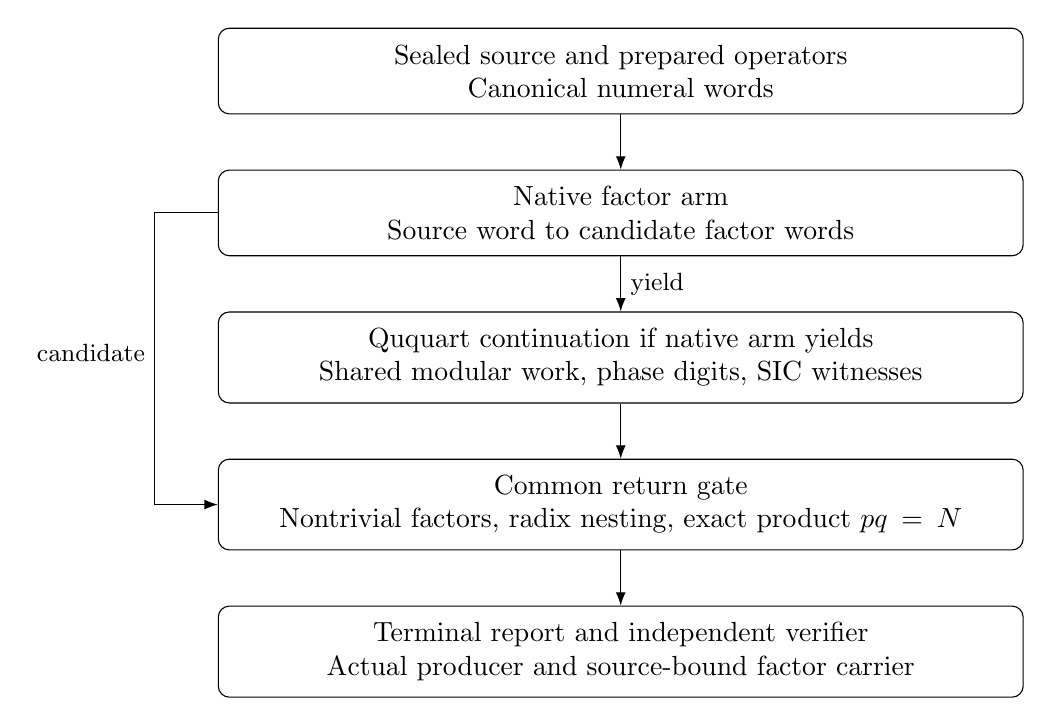
\begin{tikzpicture}[node distance=7mm,>=Latex,
box/.style={draw,rounded corners,align=center,text width=9.8cm,inner sep=6pt},
small/.style={draw,rounded corners,align=center,text width=4.3cm,inner sep=6pt}]
\node[box] (source) {Sealed source and prepared operators\\Canonical numeral words};
\node[box,below=of source] (native) {Native factor arm\\Source word to candidate factor words};
\node[box,below=of native] (phase) {Ququart continuation if native arm yields\\Shared modular work, phase digits, SIC witnesses};
\node[box,below=of phase] (gate) {Common return gate\\Nontrivial factors, radix nesting, exact product $pq=N$};
\node[box,below=of gate] (report) {Terminal report and independent verifier\\Actual producer and source-bound factor carrier};
\draw[->] (source)--(native);
\draw[->] (native)--node[right,font=\small]{yield}(phase);
\draw[->] (phase)--(gate);
\draw[->] (native.west)--++(-.8,0)|-node[pos=.24,left,font=\small]{candidate}(gate.west);
\draw[->] (gate)--(report);
\end{tikzpicture}
\caption{The implemented inclusive ordering. A successful outer arm reaches the common gate directly; the ququart and SIC continuation remains included in the prepared executable.}
\end{figure}

A decisive outer arm pays for its own production and the shared closure boundary. The continuation incurs no executed cost on that successful route. For a sequential implementation whose first success is at arm $j$, the runtime accounting is
\[
T_{\rm run}=T_{\rm load}+\sum_{i<j}T_{\rm yield,i}
+T_{\rm produce,j}+T_{\rm close}+T_{\rm report}
\]
When yielding arms return at an already determined shared boundary, their additional traversal can collapse. Placing the cheap decisive arm outermost gives the stronger case: it closes before the continuation starts. This accounting makes the nesting principle operational and leaves the yielding cost explicit for inputs on which the outer arm does work before returning.

\section*{Factor-bearing executions}

The retained source is a documented balanced, unstructured 128-bit semiprime. Both prepared radix choices use that same source. Their resolved modular bases and arithmetic nesting differ, while their phase carrier remains ququartic. Each executable returns canonical factor words. Each independent terminal verifier computes their product against its own baked copy of the source and accepts the corresponding producer schema.

\begin{center}
\begin{tabular}{@{}llll@{}}
\toprule
Work radix & Resolved base & Producing arm & Terminal product\\
\midrule
Four & Four & Native & Verified\\
Eight & Eight & Native & Verified\\
\bottomrule
\end{tabular}
\end{center}

Both completed in substantially less than one second in the retained local execution records. These timings cover the prepared executable runs, including native production and terminal release. Preparation and the separate verifier execution have their own records. The two timings are observations on one source with two preparations; a radix performance comparison requires repeated executions across a source population.

The closure audit binds the executable, embedded preparation, and verifier to their recorded digests. It confirms the exact prepared bytes are embedded, the exact returned factor-word strings are absent from the executable, and the controlled powers regenerate from the source-bound scaled base. Absence of those strings is one explicit preparation check; actual production is recorded by the executed native arm and its terminal output. The two returned factors each lie below $2^{64}$, within the native engine's documented rigorously prime factor range \cite{pari}. The product verifier independently establishes source reconstruction.

The retained native reports have zero phase shots and empty measurement ledgers. Their factor-bearing result therefore has a direct producer: the included native engine. The ququart continuation supplies its own measured-phase schema and SIC checks when reached. The complete Vox module round trip establishes a further return, from lifted module through glyphs to the identical module. Arithmetic return, measurement witnesses, and executable return each retain the object that was supplied to their instrument.

\section*{Reproduction and further construction}

The local software snapshot is G-mOMonadOS commit \texttt{00351b0}. Its retained case bundles contain the canonical source, preparation, manifest, executable, and standalone readout verifier. The companion evidence manifest to this manuscript identifies the two bundles and their terminal records. Reproduction executes a prepared membrane without arguments, saves its terminal output, and gives that output to the matching verifier. Running requires the local GP engine used by the native adapter. Source-only rebuilding additionally requires the recorded Rust and Vox preparation toolchain.

Preparation selects a canonical binary base and a power-of-two radix, resolves their modular relation, and regenerates the controlled schedule. A retained physical Fourier operator can be reused when source precision and accuracy agree. Reuse preserves the Fourier component while source-bound arithmetic powers are reconstructed. Vox then lifts the resulting executable, and a full module passes through glyph production and recovery.

The resulting architecture admits further producers without changing the multiplication obligation. Physical modular braid compilation will connect the shared-work arithmetic to the exchange substrate. Source-owned SIC inference will connect sixteen-outcome measurement to independent winding proposals. Their factor reports will cross the same return gate, carry their own producer selector, and retain the measurement witnesses actually generated on that route.

\section*{The retained numeral witness}

The following words are taken directly from the retained terminal report. Cells are broken across lines for typesetting; joining them recovers each canonical word. Both radix preparations return this pair against this source.

\noindent\textbf{Source}
\begin{flushleft}\small
⊢≻⋈∈⊥∋≻⋈∈⊥∋≻⋈∈⊥∋≻⋈∈⊥∋≻⋈∈⊤∋≻⋈∈⊤∋≻⋈∈⊤∋≻⋈∈⊤∋\\
≻⋈∈⊤∋≻⋈∈⊤∋≻⋈∈⊤∋≻⋈∈⊤∋≻⋈∈⊤∋≻⋈∈⊤∋≻⋈∈⊥∋≻⋈∈⊥∋\\
≻⋈∈⊥∋≻⋈∈⊤∋≻⋈∈⊥∋≻⋈∈⊥∋≻⋈∈⊥∋≻⋈∈⊤∋≻⋈∈⊤∋≻⋈∈⊥∋\\
≻⋈∈⊤∋≻⋈∈⊤∋≻⋈∈⊥∋≻⋈∈⊥∋≻⋈∈⊥∋≻⋈∈⊤∋≻⋈∈⊤∋≻⋈∈⊤∋\\
≻⋈∈⊥∋≻⋈∈⊤∋≻⋈∈⊤∋≻⋈∈⊥∋≻⋈∈⊥∋≻⋈∈⊤∋≻⋈∈⊤∋≻⋈∈⊥∋\\
≻⋈∈⊥∋≻⋈∈⊤∋≻⋈∈⊥∋≻⋈∈⊥∋≻⋈∈⊤∋≻⋈∈⊤∋≻⋈∈⊤∋≻⋈∈⊥∋\\
≻⋈∈⊤∋≻⋈∈⊤∋≻⋈∈⊥∋≻⋈∈⊥∋≻⋈∈⊤∋≻⋈∈⊤∋≻⋈∈⊥∋≻⋈∈⊤∋\\
≻⋈∈⊤∋≻⋈∈⊥∋≻⋈∈⊤∋≻⋈∈⊥∋≻⋈∈⊥∋≻⋈∈⊤∋≻⋈∈⊥∋≻⋈∈⊥∋\\
≻⋈∈⊤∋≻⋈∈⊥∋≻⋈∈⊥∋≻⋈∈⊤∋≻⋈∈⊤∋≻⋈∈⊥∋≻⋈∈⊥∋≻⋈∈⊤∋\\
≻⋈∈⊥∋≻⋈∈⊤∋≻⋈∈⊥∋≻⋈∈⊥∋≻⋈∈⊥∋≻⋈∈⊤∋≻⋈∈⊤∋≻⋈∈⊤∋\\
≻⋈∈⊤∋≻⋈∈⊤∋≻⋈∈⊤∋≻⋈∈⊤∋≻⋈∈⊤∋≻⋈∈⊤∋≻⋈∈⊤∋≻⋈∈⊤∋\\
≻⋈∈⊥∋≻⋈∈⊥∋≻⋈∈⊥∋≻⋈∈⊤∋≻⋈∈⊤∋≻⋈∈⊥∋≻⋈∈⊥∋≻⋈∈⊤∋\\
≻⋈∈⊤∋≻⋈∈⊤∋≻⋈∈⊥∋≻⋈∈⊥∋≻⋈∈⊥∋≻⋈∈⊥∋≻⋈∈⊤∋≻⋈∈⊥∋\\
≻⋈∈⊤∋≻⋈∈⊥∋≻⋈∈⊥∋≻⋈∈⊥∋≻⋈∈⊥∋≻⋈∈⊤∋≻⋈∈⊥∋≻⋈∈⊥∋\\
≻⋈∈⊤∋≻⋈∈⊤∋≻⋈∈⊥∋≻⋈∈⊥∋≻⋈∈⊤∋≻⋈∈⊥∋≻⋈∈⊤∋≻⋈∈⊤∋\\
≻⋈∈⊥∋≻⋈∈⊥∋≻⋈∈⊥∋≻⋈∈⊥∋≻⋈∈⊥∋≻⋈∈⊤∋≻⋈∈⊥∋≻⋈∈⊥∋⊙⊡⊣
\end{flushleft}

\noindent\textbf{First factor}
\begin{flushleft}\small
⊢≻⋈∈⊥∋≻⋈∈⊤∋≻⋈∈⊥∋≻⋈∈⊤∋≻⋈∈⊤∋≻⋈∈⊥∋≻⋈∈⊤∋≻⋈∈⊤∋\\
≻⋈∈⊥∋≻⋈∈⊥∋≻⋈∈⊤∋≻⋈∈⊤∋≻⋈∈⊥∋≻⋈∈⊤∋≻⋈∈⊤∋≻⋈∈⊤∋\\
≻⋈∈⊥∋≻⋈∈⊥∋≻⋈∈⊥∋≻⋈∈⊤∋≻⋈∈⊤∋≻⋈∈⊥∋≻⋈∈⊤∋≻⋈∈⊥∋\\
≻⋈∈⊥∋≻⋈∈⊥∋≻⋈∈⊥∋≻⋈∈⊤∋≻⋈∈⊤∋≻⋈∈⊥∋≻⋈∈⊥∋≻⋈∈⊥∋\\
≻⋈∈⊥∋≻⋈∈⊤∋≻⋈∈⊥∋≻⋈∈⊥∋≻⋈∈⊤∋≻⋈∈⊥∋≻⋈∈⊤∋≻⋈∈⊥∋\\
≻⋈∈⊤∋≻⋈∈⊥∋≻⋈∈⊤∋≻⋈∈⊤∋≻⋈∈⊤∋≻⋈∈⊥∋≻⋈∈⊥∋≻⋈∈⊤∋\\
≻⋈∈⊥∋≻⋈∈⊥∋≻⋈∈⊤∋≻⋈∈⊤∋≻⋈∈⊤∋≻⋈∈⊥∋≻⋈∈⊥∋≻⋈∈⊥∋\\
≻⋈∈⊤∋≻⋈∈⊥∋≻⋈∈⊤∋≻⋈∈⊥∋≻⋈∈⊤∋≻⋈∈⊥∋≻⋈∈⊥∋≻⋈∈⊥∋⊙⊡⊣
\end{flushleft}

\noindent\textbf{Second factor}
\begin{flushleft}\small
⊢≻⋈∈⊥∋≻⋈∈⊥∋≻⋈∈⊤∋≻⋈∈⊤∋≻⋈∈⊤∋≻⋈∈⊥∋≻⋈∈⊤∋≻⋈∈⊤∋\\
≻⋈∈⊤∋≻⋈∈⊥∋≻⋈∈⊤∋≻⋈∈⊥∋≻⋈∈⊥∋≻⋈∈⊥∋≻⋈∈⊥∋≻⋈∈⊥∋\\
≻⋈∈⊤∋≻⋈∈⊤∋≻⋈∈⊥∋≻⋈∈⊤∋≻⋈∈⊤∋≻⋈∈⊤∋≻⋈∈⊤∋≻⋈∈⊥∋\\
≻⋈∈⊥∋≻⋈∈⊤∋≻⋈∈⊥∋≻⋈∈⊤∋≻⋈∈⊥∋≻⋈∈⊥∋≻⋈∈⊥∋≻⋈∈⊥∋\\
≻⋈∈⊥∋≻⋈∈⊤∋≻⋈∈⊥∋≻⋈∈⊥∋≻⋈∈⊤∋≻⋈∈⊤∋≻⋈∈⊥∋≻⋈∈⊤∋\\
≻⋈∈⊤∋≻⋈∈⊥∋≻⋈∈⊤∋≻⋈∈⊥∋≻⋈∈⊥∋≻⋈∈⊥∋≻⋈∈⊥∋≻⋈∈⊥∋\\
≻⋈∈⊥∋≻⋈∈⊥∋≻⋈∈⊤∋≻⋈∈⊥∋≻⋈∈⊥∋≻⋈∈⊥∋≻⋈∈⊤∋≻⋈∈⊤∋\\
≻⋈∈⊥∋≻⋈∈⊥∋≻⋈∈⊤∋≻⋈∈⊤∋≻⋈∈⊥∋≻⋈∈⊥∋≻⋈∈⊥∋≻⋈∈⊥∋⊙⊡⊣
\end{flushleft}

\begin{thebibliography}{9}
\bibitem{trilattice} Y. Shramko, J. M. Dunn, and T. Takenaka, ``The Trilattice of Constructive Truth Values,'' \emph{Journal of Logic and Computation} \textbf{11}, 761--788 (2001). \href{https://doi.org/10.1093/logcom/11.6.761}{doi:10.1093/logcom/11.6.761}.
\bibitem{renes} J. M. Renes, R. Blume-Kohout, A. J. Scott, and C. M. Caves, ``Symmetric Informationally Complete Quantum Measurements,'' \emph{Journal of Mathematical Physics} \textbf{45}, 2171--2180 (2004). \href{https://arxiv.org/abs/quant-ph/0310075}{arXiv:quant-ph/0310075}.
\bibitem{appleby} D. M. Appleby, ``SIC-POVMs and the Extended Clifford Group,'' \emph{Journal of Mathematical Physics} \textbf{46}, 052107 (2005). \href{https://arxiv.org/abs/quant-ph/0412001}{arXiv:quant-ph/0412001}.
\bibitem{scott} A. J. Scott, ``Tight Informationally Complete Quantum Measurements,'' \emph{Journal of Physics A} \textbf{39}, 13507--13530 (2006). \href{https://arxiv.org/abs/quant-ph/0604049}{arXiv:quant-ph/0604049}.
\bibitem{shor} P. W. Shor, ``Polynomial-Time Algorithms for Prime Factorization and Discrete Logarithms on a Quantum Computer,'' \emph{SIAM Journal on Computing} \textbf{26}, 1484--1509 (1997). \href{https://arxiv.org/abs/quant-ph/9508027}{arXiv:quant-ph/9508027}.
\bibitem{kbs} V. Kliuchnikov, A. Bocharov, and K. M. Svore, ``Asymptotically Optimal Topological Quantum Compiling,'' \emph{Physical Review Letters} \textbf{112}, 140504 (2014). \href{https://arxiv.org/abs/1310.4150}{arXiv:1310.4150}.
\bibitem{pari} The PARI Group, \emph{PARI/GP Reference Documentation}, arithmetic functions and the factoring engine, consulted October 4, 2026. \url{https://pari.math.u-bordeaux.fr/dochtml/html/Arithmetic_functions.html}.
\end{thebibliography}
\end{document}
